\documentclass[twocolumn,10pt,a4j]{jsarticle}
\usepackage{kougai}
\usepackage{dcolumn}


\title{OffscreenCanvasを用いたシミュレータ教材の開発}
\author{1532040 岡本 悠祐  指導教員 須田 宇宙 准教授}
\date{}
 
\begin{document}
\maketitle
\section{はじめに}
シミュレータ教材は不可視現象を可視化する教材である.そのため,イメージが困難な事象の理解を促す手法として有用である.
e-Learningの普及に伴いシミュレータ教材の活用の場が増加し,様々な分野に対応したシミュレータ教材と効率的な開発手法が必要とされている.

本研究室では昨年,高負荷なシミュレータ教材にプログラマブルシェーダを利用しGPUに適用させ,CPUとの処理速度を比較する研究が行われた.その結果,教材の処理速度は大幅に向上したが,ソースコードの変更箇所が多く,複雑なため容易に実装できないという問題点が浮上した.

この問題点はWebWorkerによるマルチスレッド化と,サブスレッドから直接描画を行うOffscreenCanvasを利用することで緩和できると考られ,
そこで本研究では,OffscreenCanvasを利用したシミュレータ教材の開発を行い,ソフトウェアの生産性と処理速度の観点から有用性の検証を行うことを目的とする.

\section{開発したシミュレータ教材}
本研究ではシミュレータにおけるOffscreenCanvasの有用性の検証を行う.プログラムは昨年度本学の卒業論文である「GPU利用によるシミュレータ教材の演算速度」を拡張した\cite{book}.
\cite{book}では複数の音源から発せられる音場を表示するシミュレータを開発した.
昨年開発されたCPUとGPU向けのプログラムと,WebWorker,OffscreenCanvasを利用したシミュレータの計測を行い,それぞれを手法1,手法2,手法3,手法4と呼ぶ

図\ref{fig:sim}は実際に開発したシミュレータである.キャンバスを左右に分け,workerで処理を分散させた.

図\ref{fig:cpu}は手法1のフローチャートである.これを利用しWebWorkerとOffscreenCanvasの開発を行う.

図\ref{fig:worker}は手法3のフローチャートである.mainでworkerを定義することで,手法1をマルチスレッド化した.worker内で描画を行うことができない.

図\ref{fig:offsc}は手法4のフローチャートである.手法3を利用し,worker内での描画を可能とした.

\setlength\textfloatsep{0pt}
\begin{figure}[htbp]
\begin{minipage}{0.49\hsize}
  \centering
   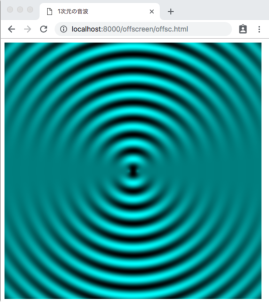
\includegraphics[width=35mm , angle=-90]{sim.pdf}
   \vspace{6pt}
  \caption{開発したシミュレータ}
  \label{fig:sim}
 \end{minipage}
 \begin{minipage}{0.49\hsize}
  \centering
   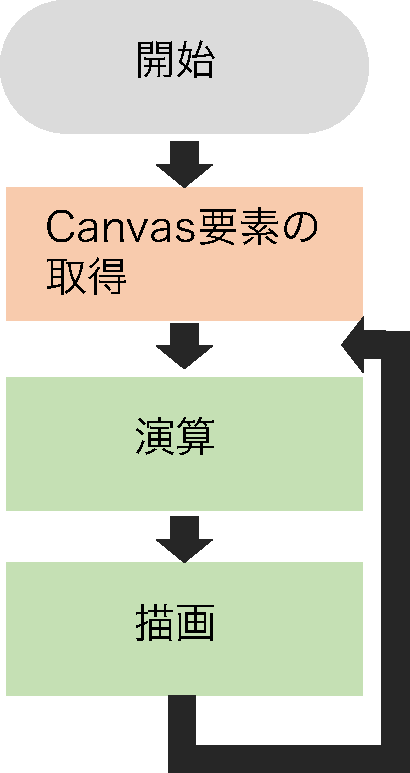
\includegraphics[width=20mm]{cpu_chart.pdf}
  \caption{手法1のフローチャート}
  \label{fig:cpu}
 \end{minipage}
 
 \begin{minipage}{0.5\hsize}
 \centering
  \vspace{5pt}	
  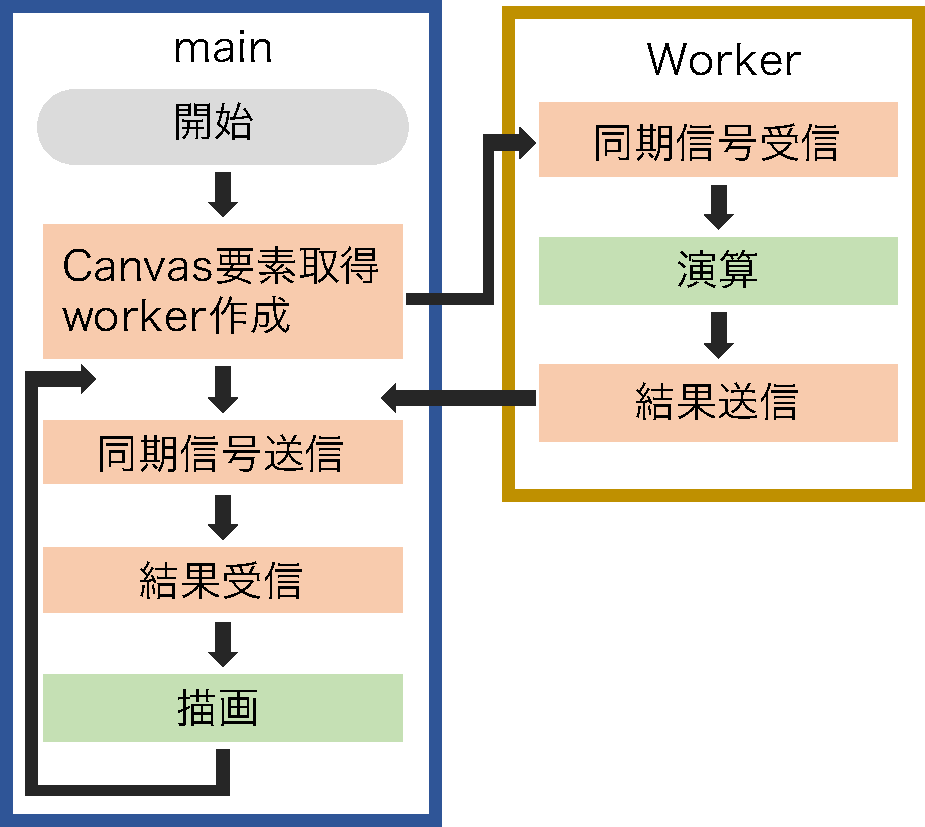
\includegraphics[width=35mm]{worker_chart.pdf}
     \belowcaptionskip=25pt
  \abovecaptionskip=5pt
  \caption{手法3のフローチャート}
  \label{fig:worker}
 \end{minipage}
 \begin{minipage}{0.5\hsize}
 \centering
 \vspace{-30pt}	
  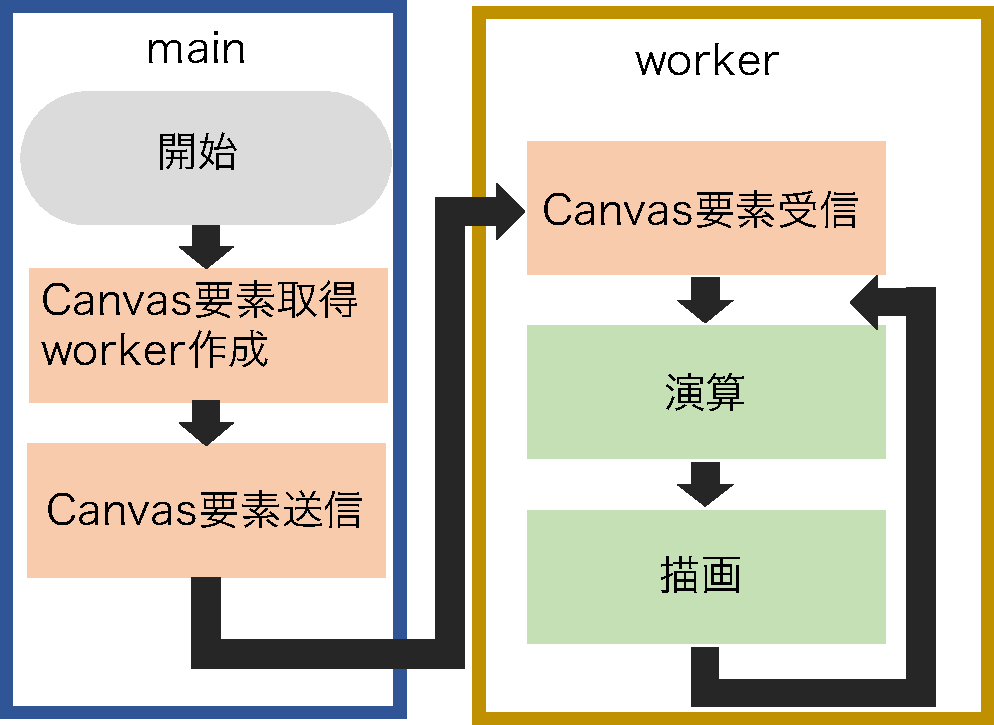
\includegraphics[width=40mm  ]{offscreen_chart.pdf}
  \abovecaptionskip=30pt
  \belowcaptionskip=-10pt
  \caption{手法4のフローチャート}
  \label{fig:offsc}
 \end{minipage}
\end{figure}

\section{検証}
4つの手法に関して処理にかかる時間や,プログラムの追加・変更箇所の比較を行い,10,000回演算を行う時間を計測した.

計測にはCPUにIntel Core i5 3.2GHz,GPUにはNVIDIA GeForce GT 775Mを搭載したパソコンを利用した.

手法1の処理に費やした時間を基準として時間比を求めた.その結果を表\ref{tab:tab2}に示す.

\begin{table} [htbp]
\centering
\vspace{-30pt}
\caption{各種法の高速化率}
\vspace{5pt}
	\begin{tabular} {| c | c | c | } \hline
	手法 & 処理時間  (s)  & 時間比 \\ \hline
	手法1 & 206.608 & 1 \\ \hline 
	手法2 & 128.652 & 0.622689 \\ \hline
	手法3 & 98.094 & 0.474786 \\ \hline
	手法4 & 164.368 & 0.795557 \\ \hline
	\end{tabular} 
	\label{tab:tab2}
\end{table}
手法1がシングルスレッドで動作するのに対し,手法3,手法4は2つのスレッドを用いて演算処理を行っているため処理速度が向上した.

図\ref{fig:cpu}・図\ref{fig:worker}・図\ref{fig:offsc}より手法3・手法4のプログラムは,mainからworkerへデータの送信を追加した.更に,手法3に関してはworkerから演算の結果をmainに送信を行う処理を追加した.
手法3は手法1の演算と描画が分離しているため,演算が終わる度に結果を送信する必要があり,mainとworker間で送受信が何度も行われた.一方手法4は,手法1の演算と描画が同じworker内で完結するため,繰り返しデータの送受信を行う必要がなく,処理1のソースコードの原型を崩すことなく移植が行えた.
プログラムの変更箇所はHTMLでキャンバスを追加,描画範囲の指定を行うことで実装できた.
\section{おわりに}
本研究ではシミュレータ開発におけるOffscreenCanvasの有用性を生産性と処理速度の観点から検証した.シングルスレッドで動作するプログラムより処理速度が向上し,WebWorkerより容易に実装が可能なことがわかった.今後は更なる処理速度の向上と,生産性の向上が求められる.
\begin{thebibliography}{99}

	\bibitem{book}中嶋 大貴:``GPU利用によるシミュレータ教材の演算速度'',平成29年度卒業論文,(2018)
\end{thebibliography}
\end{document}
